%% LyX 2.1.1 created this file.  For more info, see http://www.lyx.org/.
%% Do not edit unless you really know what you are doing.
\documentclass[12pt,english]{article}
\usepackage[T1]{fontenc}
\usepackage{float}
\usepackage{rotfloat}
\usepackage{amsthm}
\usepackage{amsmath}
\usepackage{graphicx}
\usepackage{setspace}
\usepackage[authoryear]{natbib}
\onehalfspacing

\makeatletter

%%%%%%%%%%%%%%%%%%%%%%%%%%%%%% LyX specific LaTeX commands.
%% Because html converters don't know tabularnewline
\providecommand{\tabularnewline}{\\}

\makeatother

\usepackage{babel}
\begin{document}

\section{Introduction}

During the past few decades, Uganda has experienced substantial economic
growth. Since 1986, when the National Resistance Movement took over
government, real gross domestic product (GDP) has grown at an annual
rate of 6.8 per cent, making its economy one of the fastest growing
in Africa. This growth has been attributed to the new government that
has implemented a far-reaching economic reforms agenda, transforming
Uganda into one of the most liberal economies in Africa south of the
Sahara. Indeed, as argued in World Bank (1993: 22)\nocite{WB193},
the government 'liberalized the trade regime by abolishing export
and import licensing; dismantled all price controls, which were few
to begin with; repealed the Industrial Licensing Act, promulgated
a new investment code, returned properties expropriated by the Amin
regime and commenced privatizing public industrial enterprises; made
important strides in abolishing export and distribution monopolies;
embarked upon a major overhaul of the civil service; restructured
the tax system and improved tax administration; and has made an impressive
start in restructuring public expenditures towards critical economic
and social services'. Such policy changes were seen as essential preconditions
for sustainable economic growth. 

This growth has been accompanied by equally impressive declines in
the levels of poverty as reported by the government. While aggregate
headcount poverty stood at about 57 per cent in the early 1990s, the
most recent official estimate puts 19.5 per cent of the population
below the official poverty line.%
\footnote{For the most recent official estimate, we take the poverty estimate
based on the 2012/13 Uganda National Household Survey (UNHS). The
data on which these estimates are based were obtained from the Uganda
Bureau of Statistics (UBOS) in August 2014. As is mostly the case
with UNHS data obtained from UBOS, the dataset came with a compiled
welfare aggregate based on consumption expenditure and a set of official
poverty lines. Using the same methods we used to replicate official
poverty figures in previous rounds of the UNHS, we estimate national
headcount poverty to be 19.5 per cent in the UNHS 2012/13. This is
slightly lower than official poverty estimates at the time of the
UNHS 2012/13 dissemination and reported in the press (22.1 per cent). %
} But despite these successes at the aggregate level, researchers warn
that this growth has not been shared equally by the population at
large. For instance, marked spatial heterogeneity in baseline poverty
and subsequent poverty reductions mean that differences in the standard
of living between locations are often much higher now than what they
used to be. 

Apart from the observed heterogeneity in terms of poverty and poverty
reduction, the figures itself have been called into question as well.
Some argue that the lack of progress on assets accumulation and non-monetary
well-being proxies suggest much more modest poverty reductions, raising
suspicion about the poverty lines and the welfare indicator used by
the government of Uganda (\citealt{New10,New4}). Some scholars have
also been questioning the spatial pattern of poverty as reported in
official documents, arguing that a single national food poverty line
is likely to overstate poverty in some areas while underestimating
poverty in others (\citealt{RePEc:oup:jafrec:v:12:y:2003:i:4:p:598-624,New1}). 

In this paper, we want to update existing knowledge about the state
of poverty and its dynamics in Uganda, while at the same time address
some of the problems with the official figures that have been identified
in recent studies. To account for differences in diets in different
locations, we will construct different poverty thresholds for different
spatial domains using the latest available nationally representative
household survey (UNHS 2012/13). For each spatial domain, we construct
a food basket that produces a certain minimum of calories that reflects
the diets of the poorest households in that region. These baskets
are then multiplied by prices prevailing in that region to arrive
at food poverty lines. An allowance for basic non-food necessities
is then added to get a set of Cost of Basic Needs (CBN) poverty lines,
one in each spatial domain. We then test these poverty lines to see
if they are utility-consistent. The idea is that a basic needs bundle
in a certain spatial domain A should always be cheaper than a bundle
from any other region valued at prices of region A. If a bundle does
not satisfy these revealed preference conditions, we use an information
theoretic approach to adjust the bundles until they do, as outlined
in \citet{RePEc:ucp:ecdecc:v:58:y:2010:i:3:p:449-474}. 

While comparing poverty estimates using these new poverty lines with
the official estimates is interesting in its own right, we will use
the utility-consistent poverty lines to look at poverty dynamics using
the recently released Uganda National Panel Survey (UNPS). The UNPS
is a yearly panel survey collected by the Uganda Bureau of Statistics
(UBOS) supported by the World Bank's Living Standard Measurement Study
(LSMS) project that tracks about 3,000 households. We can use the
panel nature of this survey to study how many households are chronically
poor (defined as always falling below the poverty threshold) and investigate
how their characteristics differ from other groups, such as households
that successfully escaped poverty. In other words, we will construct
a detailed poverty profile that takes dynamic aspects into account,
defining groups based on poverty transitions instead of a simple dichotomous
poor/non-poor status (\citealt{Boateng01031992}). As for the characteristics
we contrast within each group, we confine ourselves to those that
change only slowly over time, and we look at the ``initial conditions''
at the start of the panel. We hope that this can enlighten us on the
preconditions that need to be in place to be in a particular poverty
dynamics group.%
\footnote{For example, we could check if households that are always below the
poverty line are different in terms of their reported ability to cope
with adverse shocks at the start of the panel from those that grow
out of poverty over the course of the panel.%
} 

The remainder of this paper is structured as follows: We first give
an overview of poverty in the past few decades and look at the present
official poverty estimates in Uganda. We also present some studies
that point to shortcomings in official poverty measurement. In Section
3, we briefly explain the reasoning behind the use of spatially disaggregated
poverty lines and the role of revealed preferences to test for utility
consistency. Section 4 presents the construction of the new set of
poverty lines and our poverty estimates based on the UNHS 2012/13.
Section 5 then looks at poverty dynamics and relates households with
differing poverty dynamics to a selection of characteristics. A final
section concludes. 


\section{Poverty in Uganda: Trends and controversies}

During the 1990s, poverty in Uganda decreased substantially, falling
by almost 40 per cent at the national level. Table 2 in \citet{RePEc:oup:jafrec:v:12:y:2003:i:4:p:598-624}
presents official headcount poverty rates before the year 2000.%
\footnote{There is a substantial literature on poverty and its dynamics in the
1990s. This is because of the relatively high quality data available
for this period. Uganda has been conducting national household surveys
since 1992, and conducted six such surveys before the turn of the
millennium. Some of these datasets form a panel. The first dataset,
the Integrated Household Survey conducted in 1992/1993 can be linked
to the last survey of the millennium, referred to as the first Uganda
National Household Survey (UNHS 1999/2000). Between these two surveys,
a series of four Monitoring Surveys (1993/1994 up to 1997/1998) was
carried out. More information on these data sets can be found in \citet{RePEc:taf:jdevst:v:42:y:2006:i:7:p:1225-1251}.%
} The table also shows significant spatial differences in both levels
and changes in poverty. The urban areas and central region reduce
poverty the fastest. The northern region, already starting from high
levels of poverty, is relatively unsuccessful in bringing down the
number of people living below the poverty line. In addition, studies
that exploit the panel nature of the data find that in some regions,
poverty is particularly persistent (\citealt{DPR:DPR220}). Also puzzling
is the sudden drop between 1997/1998 and 1999/2000. Although it took
five years for poverty to decrease by 20 per cent between 1992 and
1997, it took only two years to decrease another 20 per cent at the
turn of the century. This may be due to inconsistent underlying welfare
indicator data that were obtained from different surveys (the Monitoring
Surveys and the Uganda National Household Survey, see footnote 3).

One controversy we will also address in this paper refers to the fact
that the official poverty estimates are based on poverty lines that
are rooted in a single food consumption bundle, derived from 1993/1994
Monitoring Survey data. In particular, a single food basket was identified
at the national level with 28 of the most frequently consumed food
items by households with less than the median income. The items in
this food basket were then converted into caloric equivalents and
scaled to generate 3,000 calories per adult equivalent per day using
the World Health Organization (WHO) estimates for an 18-30-year-old
male as a reference. Next, a non-food allowance was added. Non-food
requirements were estimated as the average non-food expenditure of
those households whose total expenditure was around the food poverty
line. The non-food allowance does allow for spatial heterogeneity,
as separate averages were calculated for urban and rural locations
interacted with the four regions (central, eastern, northern, and
western), using the method described in \citet{RePEc:oup:wbecrv:v:8:y:1994:i:1:p:75-102}.
As far as we know, these poverty lines have since been updated by
the official inflation figures each time a new household survey came
out.

\citet{RePEc:oup:jafrec:v:12:y:2003:i:4:p:598-624} and \citet{New1}
argue that Uganda is unusual in its dietary diversity. Indeed, Uganda
has five different staples, matooke, maize, sweet potatoes, cassava,
and millet that are more or less important within the diet depending
on the region. This may not matter very much if the diets are equally
cost-effective in obtaining the same level of basic needs as defined
in kilo-calories. However, the staple food of choice of a large part
of the population, both in the western and the central regions, is
matooke, a highly localized staple.%
\footnote{Matooke is a variety of starchy banana, commonly referred to as cooking
bananas.%
} \citet{RePEc:oup:jafrec:v:12:y:2003:i:4:p:598-624} calculates that,
at least in 1993-1994, matooke appeared to be a very expensive source
of calories, compared with what people in, for instance, the north
consume. When \citet{RePEc:oup:jafrec:v:12:y:2003:i:4:p:598-624}
and \citet{New1} account for this in their analysis, they come to
the conclusion that poverty is more pronounced in the western region
than found in official statistics. Even after correcting for income
difference, as regions that consume more expensive calories may do
so simply because they have higher incomes, \citet{RePEc:oup:jafrec:v:12:y:2003:i:4:p:598-624}
comes to the conclusion that the western region overtakes even the
northern region as the poorest. 

Progress in fighting poverty reported by the government of Uganda
and UBOS in the first decade of the new millennium is equally impressive.
Table \ref{tab:Official-poverty-headcount00s} shows that poverty
at the national level kept falling during the first decade, shaving
another 50 per cent off of headcount poverty. At the same time, differential
progress in poverty reduction in different regions persists, too.
For instance, by 2012/13, poverty is more than eight times higher
in the northern region than in the central region. In 2002/2003, the
north was only 2.7 times poorer than the central region. The more
disaggregated the numbers, the starker the contrasts become. In the
northeast, a semi-arid area with low rainfall inhabited by the Karamajong,
an agro-pastoralist ethnic group, poverty remains stubbornly high,
while in the central and western regions of the country, poverty is
almost eradicated.%
\footnote{The northeastern subregion includes the districts of Kotido, Moroto,
Nakapiripiriti, Katwaki, Amuria, Soroti, Kumi, and Kaberamaido; mid-northern
includes Gulu, Kitgum, Pader, Apac, and Lira; West Nile includes Moyo,
Adjumani, Yumbe, Arua, Koboko, and Nebbi; mid-western includes Masindi,
Hoima, Kibaale, Bundibugyo, Kabarole, Kasese, Kyenjojo and Kamwenge;
southwestern includes Bushenyi, Rukungiri, Kanungu, Kabale, Kisoro,
Mbarara, and Ntungamo; eastern includes Kapchorwa, Mbale, Tororo,
Sironko, Paliisa, and Busia; central 1 includes Kalangala, Masaka,
Mpigi, Rakai, Sembabule, and Wakiso; Central 2 includes Kayunga, Kiboga,
Luwero, Mubende, Mukono, and Nakasongola; East Central includes Jinja,
Iganga, Kamuli, Bugiri, and Mayuge. %
}

\begin{table}
\protect\caption{Official poverty headcounts 2002-12\label{tab:Official-poverty-headcount00s}}


\begin{centering}
\begin{tabular}{lcccc}
\hline 
 & 2002/03 & 2005/06 & 2009/10 & 2012/13\tabularnewline
\hline 
\hline 
Uganda & 38.8 & 31.1 & 24.5 & 19.5\tabularnewline
 &  &  &  & \tabularnewline
Urban & 14.4 & 13.7 & 9.1 & 9.6\tabularnewline
Rural & 42.7 & 34.2 & 27.2 & 22.4\tabularnewline
 &  &  &  & \tabularnewline
Central & 22.3 & 16.4 & 10.7 & 5.1\tabularnewline
Eastern & 46.0 & 35.9 & 24.3 & 24.1\tabularnewline
Northern & 63.0 & 60.7 & 46.2 & 43.7\tabularnewline
Western & 32.9 & 20.5 & 21.8 & 7.6\tabularnewline
 &  &  &  & \tabularnewline
Kampala & 4.7 & 4.4 & 3.9 & 0.8\tabularnewline
Central 1 & 22.0 & 18.8 & 11.1 & 3.9\tabularnewline
Central 2 & 30.0 & 19.7 & 13.6 & 7.9\tabularnewline
East Central & 42.6 & 32.7 & 21.4 & 24.1\tabularnewline
Eastern & 48.4 & 39.2 & 26.5 & 24.1\tabularnewline
Mid-northern & 57.4 & 61.1 & 40.4 & 35.6\tabularnewline
Northeastern & 82.8 & 79.3 & 75.8 & 74.5\tabularnewline
West Nile & 62.8 & 55.3 & 39.7 & 42.0\tabularnewline
Mid-western & 37.9 & 23.2 & 25.3 & 9.5\tabularnewline
Southwestern & 29.0 & 18.7 & 18.4 & 5.8\tabularnewline
\hline 
\end{tabular}
\par\end{centering}

\centering{}Source: Figures are calculated from the respective UNHS. 
\end{table}


The official poverty figures have been questioned in recent years
for being overly optimistic. \citet{New10} use Demographic and Health
Survey (DHS) data and methods related to poverty mapping and small
area estimation to look at poverty trends across Uganda from 1995
to 2010. They use the 2005/06 UNHS survey to estimate regressions
that correlate poverty to a range of household characteristics that
also appear in the DHS (four such surveys have been carried out between
1995 and 2009/10). They then use the DHS surveys to predict poverty
in each of the DHS survey years. They find that poverty indeed reduced
over time, but much slower than official figures suggest. While their
national estimate of headcount poverty in 2006 is 33 per cent and
thus very close to the official estimate of 2005/06, the rate still
stands as 30 per cent using the 2009 DHS, about 6 percentage points
higher than the 2009/10 UNHS estimate.

This view is shared among many publicists and opinion makers in Uganda.
\citet{New3} calls officially reported poverty changes ``a fiction.''
\citet{New4} admits that qualitative findings on poverty trends suggest
there was a decrease in well-being despite the drop in poverty rates.
Recently, an unpublished manuscript has been circulating that compares
Uganda to other African countries on six non-monetary poverty indicators,
such as literacy rates and access to piped water. This admittedly
partial analysis also points to a much higher incidence of poverty
than officially reported.


\section{Utility-consistent poverty lines using revealed preferences}

From the above, we learn that one of the main weaknesses of the official
poverty measures is that they are based on a poverty line that is
constructed using a single food commodity bundle for the entire country.
In addition, this food basket was constructed in 1993 and has not
been updated since, apart from accounting for simple inflation by
the consumer price index. However, it is well known that in many instances
- for example, if relative prices of basic commodities vary by region
(or through time) and preferences permit substitution - the use of
a single consumption bundle may yield inconsistent poverty comparisons
(\citealt{RePEc:ucp:ecdecc:v:51:y:2002:i:1:p:77-108}). While differences
in prices in different locations are usually incorporated in poverty
measurement by adjusting the welfare indicator to reflect prices used
in the construction of the poverty lines (or by adjusting the poverty
lines to reflect prices used in the construction of the welfare indicator),
it is becoming more and more common to also account for spatial heterogeneity
in consumption bundles in an effort to increase the \emph{specificity}
of poverty lines (e.g. \citealt{RePEc:bla:revinw:v:52:y:2006:i:3:p:399-421};
\citealt{RePEc:eee:wdevel:v:31:y:2003:i:2:p:339-358}).

While differences in consumption baskets are interesting in their
own right, they become relevant only in the context of poverty measurement
and analysis, as we relate a welfare indicator to the cost of these
basic needs. Indeed, different diets may provide the same basic needs
(usually a given amount of kilo-calories per day) at significantly
different costs, which complicates poverty comparisons between units
(regions, households, individuals, and so forth) with different diets.
It is especially in this regard that Uganda provides an interesting
study. Matooke, the main ingredient in the diet of households in the
west, may be more or less expensive per energy unit than, for example,
sorghum, the main staple in the north. As such, it would be misleading
to compare the west with the north on the basis of a single food poverty
line, even after allowing for spatial price heterogeneity.

But how can we be sure that two different consumption bundles provide
the same basic needs? Or, in the language of \citet{RePEc:oup:wbecrv:v:8:y:1994:i:1:p:75-102},
how do we ensure \emph{consistency}%
\footnote{A poverty measure is consistent if two individuals at the same welfare
level are considered equally poor. %
}? The theory underlying absolute poverty lines is grounded in welfare
economics and constrained utility maximization. In this context, the
fixed standard of living represented by the poverty line is viewed
as a level of utility associated with the minimally acceptable standard
of living. Different poverty lines will be utility-consistent if the
underlying bundles of goods are on the Hicksian utility-compensated
demand functions and hence yield the same level of utility (\citealt{RePEc:ucp:ecdecc:v:58:y:2010:i:3:p:449-474}).
In other words, two bundles of goods are consistent if they yield
the same utility. As \citet{RePEc:bla:revinw:v:52:y:2006:i:3:p:399-421}
argue, the theory of revealed preferences provides a framework for
answering these questions. 

The idea uses the rationality assumption that economic agents that
derive utility from consumption always prefer consuming more to less.
Let us assume that a representative agent living in spatial domain
\emph{$(r\in R)$ }derives utility from a set of consumption goods
($i\in I$). We will then instruct each representative consumer in
each spatial domain \emph{r }to spend a minimum to attain an arbitrary
(but constant across spatial domains) level of utility. As such, each
individual will spend $\sum p_{i,r}q_{i,r}$ on a consumption bundle,
with $p_{i,r}$ the price of good \emph{i} in spatial domain \emph{r}
and $q_{i,r}$ the quantity of good \emph{i} in spatial domain \emph{r}.
Revealed preference conditions will then imply that

\begin{equation}
\sum p_{i,r}q_{i,r'}\geq\sum p_{i,r}q_{i,r}\;\forall r,r'.\label{eq:revpref}
\end{equation}


This is so because the representative consumer in spatial domain \emph{r}
will choose only that bundle that minimizes expenditure. Thus, any
other bundle that yields the same level of utility (such as, for instance,
the one chosen by the representative consumer in region \emph{r'})
should be equally expensive as or more expensive than the chosen bundle.
No bundle can cost less than the chosen one yet yield that same utility,
because then the rational consumer should have chosen that one. Or,
as in \citet{RePEc:ucp:ecdecc:y:2003:v:52:i:1:p:159-85}, if the cost
of a bundle from another domain would be cheaper if bought in a specific
domain, this means it must have lower utility than the bundle in that
specific domain, as otherwise the rational consumer would have picked
the bundle from the other domain. The above condition \eqref{eq:revpref}
should hold for all possible pairs of spatial domains.

In practice, however, it will be hard to construct a set of poverty
lines that meet revealed preference conditions for all possible pairs
of spatial domains. One approach, which we will use in this paper,
uses a minimum cross-entropy approach to adjust expenditure shares
such that they meet revealed preference conditions (\citealt{RePEc:ucp:ecdecc:v:58:y:2010:i:3:p:449-474}).
This approach uses the expenditure shares of the original bundles
as prior information (in the form of probabilities that an arbitrarily
small amount of money will be devoted to the purchase of the particular
good) and the revealed preference conditions as constraints on the
values that the parameters can take. The end result will be a set
of adjusted expenditure shares that are as close as possible to the
original shares, yet that obey a minimal set of conditions such that
the estimated bundles are consistent with some arbitrary unknown preference
set. 


\section{A reassessment of poverty in Uganda}

In this reassessment of poverty in Uganda, we will mainly work with
the four waves of the Uganda National Panel Survey (UNPS). The UNPS
is a multi-topic panel household survey started by UBOS in 2009/10.
However, the 2009/10 sample was essentially a subset of 3,123 households
that were interviewed as part of the 2005/06 Uganda National Household
Survey (UNHS 2005/06), a nationally representative survey that covered
6,775 households. As such, the first wave of the panel comprises the
UNHS 2005/06 data of this subsample of 3,123 households. After the
second wave of 2009/10, the survey was repeated annually. Currently
data are available for a third round covering the 2010/11 agricultural
year and a fourth round covering the 2011/12 agricultural year.%
\footnote{No UNPS survey has been done in 2012/13.%
} The UNPS is conducted in two visits to better capture agricultural
outcomes associated with the two cropping seasons of the country.
More information about the UNPS can be found in \citet{UBOSBID}.

For the construction of the utility-consistent poverty thresholds
elaborated on in the previous section, we will use the 2012/13 Uganda
National Household Survey (UNHS 2012/13). Just as the UNHS 2005/06,
the UNHS 2012/13 is nationally representative, this time covering
6,888 households. We choose this survey because it is the most recent
one available, and the construction of utility-consistent poverty
lines requires a sufficiently large sample, with sufficient observations
in each spatial domain. The larger dataset allows us to experiment
with different degrees of spatial disaggregation for the domains.
It also allows us to define poverty lines at a more disaggregated
level than the maximum level of disaggregation for which the UNPS
is deemed representative.%
\footnote{The UNPS is representative only up to the regional level.%
} Our baseline case will look at poverty measures based on a single
national poverty line using a single spatial domain, as this would
be close to simply updating the current official poverty line. This
will then be compared to an analysis based on six separate spatial
domains (Kampala, Rural central, Rural East, Rural North, Rural West,
and Other Urban).

More specifically, following \citet{RePEc:ucp:ecdecc:v:58:y:2010:i:3:p:449-474},
we start by constructing food bundles in each spatial domain. In each
domain, a basket of food products that satisfies basic calorie needs
is identified using information on the age and sex composition of
the households and the recorded consumption patterns of poorer households.%
\footnote{The demographic structure of each region is mapped to an average basic
calorie requirement in each region using \citet{WHO1985}. The mapping
from these basic caloric needs into basic needs consumption bundles
is based on \citet{FAO1968}. %
} The cost of this basket, valued at prices prevailing within each
spatial domain, results in a set of food poverty lines, one in each
spatial domain. non-food poverty lines are obtained by calculating
the share of food expenditures for households whose total food and
non-food consumption per capita is near the food poverty line. Total
poverty lines are obtained as the sum of the food and the non-food
poverty lines. These poverty lines are then compared, to make sure
that they are utility-consistent. In particular, we compare the cost
of a bundle in one spatial domain to the bundles in the other spatial
domains, but evaluated at the price in this spatial domain. As stated
above, revealed preferences states that the cost of the bundle in
the spatial domain should be smaller or equal to the bundles chosen
in any other spatial domain. If this condition is violated, we use
a minimum cross-entropy framework to adjust consumption shares in
such a way that revealed preference conditions are satisfied.

It can be instructive to have a closer look at the poverty lines.
After all, poverty lines are not only useful to separate the rich
from the poor, but also serve as deflators for cost-of-living differences,
permitting interpersonal welfare comparisons when the cost of acquiring
basic needs varies over time or space (\citealt{RePEc:fth:wobali:133}).
Table \ref{tab:Utility-consist} reports the utility-consistent poverty
lines we estimate using the 2012/13 UNHS based on the six different
spatial domains.%
\footnote{The poverty lines in Table \ref{tab:Utility-consist} are aggregated
to different spatial domains for the sake of comparison to official
statistics. The underlying poverty lines for the six spatial domains,
in addition to a poverty line using only one (national) spatial domain
for comparison, are presented in Table \ref{tab:Utility-Consistent-Poverty}
in the appendix. It is not possible to directly compare the utility-consistent
poverty lines we estimate to the official poverty lines, since spatial
price differences are not reflected in the poverty lines. Instead,
the official poverty measures incorporate spatial price difference
by adjusting the welfare indicator.%
} The cost of living seems to be highest in the central region. The
Western region comes in second. This is consistent with the findings
of \citet{RePEc:oup:jafrec:v:12:y:2003:i:4:p:598-624} and \citet{New1}
and is caused by the low energy content and relatively high price
of matooke, a staple grown and consumed mostly in the western and
central regions. Households in the eastern region, on the other hand,
consume a lot of cassava, mostly in dried or flour form, which is
only three times as costly but more than eight times as nutritious.
While the 2012/13 poverty lines are directly derived from the 2012/13
UNHS, the poverty lines for the other years are simply deflated using
the Consumer Price Index. Poverty lines are expressed in Ugandan shillings
per person per day.

\begin{table}
\protect\caption{Utility-consistent poverty lines based on UNHS 2012/13\label{tab:Utility-consist}}


\begin{centering}
\begin{tabular}{lccccc}
\hline 
 & \multicolumn{1}{c}{2005/06} & \multicolumn{1}{c}{2009/10} & 2010/11 & 2011/12 & 2012/13\tabularnewline
\cline{2-6} 
Uganda & 929.34 & 1338.13 & 1425.52 & 1760.93 & 1860.54\tabularnewline
 &  &  &  &  & \tabularnewline
Rural & 901.93 & 1298.66 & 1383.47 & 1708.99 & 1805.66\tabularnewline
Urban & 1024.69 & 1475.43 & 1571.78 & 1941.61 & 2051.44\tabularnewline
 &  &  &  &  & \tabularnewline
Central & 1048.57 & 1509.80 & 1608.40 & 1986.84 & 2099.23\tabularnewline
Eastern & 798.40 & 1149.59 & 1224.66 & 1512.81 & 1598.39\tabularnewline
Northern & 914.35 & 1316.54 & 1402.52 & 1732.52 & 1830.52\tabularnewline
Western & 975.27 & 1404.26 & 1495.96 & 1847.95 & 1952.49\tabularnewline
 &  &  &  &  & \tabularnewline
Kampala & 1262.39 & 1817.68 & 1936.38 & 2392.00 & 2527.30\tabularnewline
Central 1 & 1013.24 & 1458.94 & 1554.21 & 1919.91 & 2028.51\tabularnewline
Central 2 & 1020.24 & 1469.02 & 1564.95 & 1933.17 & 2042.53\tabularnewline
East Central & 803.39 & 1156.78 & 1232.33 & 1522.28 & 1608.39\tabularnewline
Eastern & 794.83 & 1144.45 & 1219.19 & 1506.05 & 1591.25\tabularnewline
Mid-northern & 917.31 & 1320.81 & 1407.07 & 1738.14 & 1836.46\tabularnewline
Northeastern & 911.04 & 1311.78 & 1397.45 & 1726.26 & 1823.91\tabularnewline
West Nile & 910.74 & 1311.34 & 1396.98 & 1725.68 & 1823.30\tabularnewline
Mid-western & 975.58 & 1404.72 & 1496.45 & 1848.55 & 1953.12\tabularnewline
Southwestern & 974.96 & 1403.82 & 1495.50 & 1847.38 & 1951.88\tabularnewline
\hline 
\end{tabular}
\par\end{centering}

\centering{}Source: Figures are calculated from the respective UNHS
2012/13. 
\end{table}


Let us now look at the evolution of poverty during the recent past.
We will present two sets of results. The first set of results, reported
in Table \ref{tab:Poverty-headcounts-1spdomain}, uses only one spatial
domain. In other words, we estimate a single national poverty line
based on a single national food basket.%
\footnote{This national poverty line was estimated to be 1233.42, see first
row in Table \ref{tab:Utility-Consistent-Poverty} in the appendix.
One may be surprised that the poverty line based on a single spatial
domain is so low, and below all of the other poverty lines estimated
in the six regions, instead of somewhere in between. This is because,
using only one spatial domain essentially means that a single poverty
line is constructed based on the lowest cost and lowest consuming
rural zones. This leads to a low poverty line, closer to the lowest
poverty line using different spatial domains (eastern region) than
to the highest poverty line (Kampala). The fact that the poverty line
using one spatial domain is actually below the lowest poverty line
when different spatial domains are used is due to the utility consistency
adjustments. Poverty lines for the central and eastern regions are
significantly adjusted upward, lifting them above the poverty line
using a single spatial domain. %
} We do this because, in a way, this would be the closest to simply
updating the official poverty line, that is based on one single national
consumption basket. Second, we will present results for an analysis
that uses the six spatial domains mentioned above (Kampala, Rural
Central, Rural East, Rural North, Rural West, and Other Urban). The
results are reported in Table \ref{tab:Poverty-headcounts-6spdomains}.

\begin{table}
\protect\caption{Poverty headcounts 2002-2012 using one spatial domain\label{tab:Poverty-headcounts-1spdomain}}


\begin{centering}
\begin{tabular}{lcccccccccc}
\hline 
 & \multicolumn{2}{c}{2005/06} & \multicolumn{2}{c}{2009/10} & \multicolumn{2}{c}{2010/11} & \multicolumn{2}{c}{2011/12} & \multicolumn{2}{c}{2012/13}\tabularnewline
 & P0 & contr & P0 & contr & P0 & contr & P0 & contr & P0 & contr\tabularnewline
\hline 
\hline 
Uganda & 0.216 & 1.000 & 0.200 & 1.000 & 0.207 & 1.000 & 0.157 & 1.000 & 0.136 & 1.000\tabularnewline
 &  &  &  &  &  &  &  &  &  & \tabularnewline
Rural & 0.250 & 0.965 & 0.229 & 0.963 & 0.232 & 0.962 & 0.179 & 0.951 & 0.159 & 0.900\tabularnewline
Urban & 0.046 & 0.035 & 0.047 & 0.037 & 0.056 & 0.038 & 0.045 & 0.049 & 0.060 & 0.100\tabularnewline
 &  &  &  &  &  &  &  &  &  & \tabularnewline
Central & 0.103 & 0.148 & 0.082 & 0.127 & 0.048 & 0.059 & 0.022 & 0.031 & 0.024 & 0.046\tabularnewline
Eastern & 0.223 & 0.257 & 0.200 & 0.244 & 0.248 & 0.321 & 0.186 & 0.379 & 0.165 & 0.352\tabularnewline
Northern & 0.488 & 0.390 & 0.385 & 0.346 & 0.300 & 0.335 & 0.286 & 0.382 & 0.336 & 0.512\tabularnewline
Western & 0.164 & 0.205 & 0.212 & 0.283 & 0.240 & 0.285 & 0.129 & 0.207 & 0.051 & 0.090\tabularnewline
\hline 
\end{tabular}
\par\end{centering}

\begin{centering}
Source: Figures are calculated from the respective UNHS and UNPS waves.
\par\end{centering}

\centering{}Note: P0 means headcount poverty, contr means contribution
to national poverty. 
\end{table}


Poverty headcounts using one spatial domain as reported in Table \ref{tab:Poverty-headcounts-1spdomain}
are much lower than the official headcounts reported in Table \ref{tab:Official-poverty-headcount00s}.
For instance, the national estimate in 2005/06 is about 10 percentage
points lower than the official estimates. However, the reduction in
poverty between 2005/06 and 2009/10 (7.4 per cent) is much smaller
than in the official figures (more than 20 per cent). There is a slight
increase in poverty in 2010/11, but national headcount poverty falls
to about 16 per cent in 2011/12.%
\footnote{While part of the increase in 2010/11 is likely caused by the increase
in food prices, data problems provide an additional explanation. For
instance, simple counts of how many households report consuming a
particular commodity point to some severe problems. In 2010/11 only
about 300 household report consuming sweet potatoes, while this is
around 1,400 in the other rounds. For cassava, in 2010/11 only 562
household report consumption, versus again about 1,400 in all other
rounds of the UNPS.%
} Overall, the reduction in poverty between 2005/06 and 2012/13 was
about the same as in the official figures at around 37 per cent, most
of this coming about in the two last years of the panel. The spatial
patterns are the same, as both these and the official estimates are
based on a single poverty line.

The national poverty headcounts are much higher than the official
ones if we use six spatial domains (Table \ref{tab:Poverty-headcounts-6spdomains}).
While \citet{New10} argue that the original 1993 poverty lines may
have increased too little to keep pace with inflation and that differences
in the measurement of consumption may contribute to the underestimation
of poverty, we find that consumption bundle aggregation also seems
to depress poverty figures. The reductions in poverty also seem more
modest than the official ones, with an overall reduction in poverty
between 2005/06 and 2012/13 of about one quarter. We also see that
the largest reduction the number of people living below the poverty
line happened between 2011/12 and 2012/13. However, if we look at
the evolution of the poverty gap (as reported in Table \ref{tab:Poverty-gap-2002-2012}
in the Appendix), the largest reduction is between 2010/11 and 2011/12.
This suggests quite some mobility below the poverty line between 2010/11
and 2011/12.

If we disaggregate between rural and urban poverty, we see that most
of the poverty reduction has been happening in rural areas. Over the
years, poverty in rural areas has steadily fallen from almost 50 per
cent to 36 per cent. This is different from what has been happening
in urban areas. While between 2005/06 and 2010/11 urban poverty was
on the decline, it started rising again afterwards. A marked acceleration
in urban poverty between 2011/12 and 2012/13 together with a steady
decline in rural poverty reduced the contribution of rural poverty
to overall poverty from about 94 per cent to 88 per cent in 2012/13.
The evolution of official figures is in line with our findings, except
that we find a much stronger rebound of urban poverty.

Finally, we disaggregate poverty by region. We find that in the Northern
region, which is the poorest, poverty has decreased by 15 per cent
over the entire period. However, the evolution was far from linear.
Especially between 2009/10 and 2010/11, there was a strong reduction
in poverty. But since then, poverty in the northern region has been
rising again. The tables in the appendix show that, especially in
2012/13, not only headcount poverty but also the poverty gap and the
severity of poverty has been increasing. Official poverty figures
report a reduction of 28 per cent between 2005/06 and 2012/13 in headcount
poverty, very close to what we find using only one spatial domain
(figure \ref{tab:Poverty-headcounts-1spdomain}). The western region
is, just as in the official estimates, the second richest region.
However, it is now 55 per cent poorer than the richest region. This
gap between the western and central regions is significantly larger
than in the official statistics, where poverty rates in the western
region are 33 per cent higher than in the eastern region. Thus, while
we do not observe the changes in the rankings observed by \citet{RePEc:oup:jafrec:v:12:y:2003:i:4:p:598-624},
our results are consistent with the finding that the west is poorer
than official figures suggest.

The central region, already the least poor region at the start of
the panel, reduced headcount poverty by half between 2005/06 and 2012/13
according to our estimates using six spatial domains. Again, official
estimates record higher poverty reductions (almost 70 per cent), which
is again similar to what we find in our estimates using only one spatial
domain. Inequality in poverty headcount has also increased over time.
While the northern region initially contributed 27 per cent to overall
poverty, this has increased to 37 per cent in 2012/13. The contribution
of the eastern region also has increased substantially. And while
severity of poverty has reduced in the northern region, in 2012/13,
almost 60 per cent of the national severity of poverty measure was
contributed by the North. If we disaggregate the 2012/13 data further,
we find that most poverty is found in the northeast, where over 80
per cent of the individuals live in poverty. This is followed by West
Nile, a distant second with 60 per cent of the population living in
poverty. 

\begin{table}
\protect\caption{Poverty headcounts 2002-2012 using six spatial domains\label{tab:Poverty-headcounts-6spdomains}}


\begin{centering}
\begin{tabular}{lcccccccccc}
\hline 
 & \multicolumn{2}{c}{2005/06} & \multicolumn{2}{c}{2009/10} & \multicolumn{2}{c}{2010/11} & \multicolumn{2}{c}{2011/12} & \multicolumn{2}{c}{2012/13}\tabularnewline
 & P0 & contr & P0 & contr & P0 & contr & P0 & contr & P0 & contr\tabularnewline
\hline 
\hline 
Uganda & 0.423 & 1.000 & 0.381 & 1.000 & 0.370 & 1.000 & 0.359 & 1.000 & 0.315 & 1.000\tabularnewline
 &  &  &  &  &  &  &  &  &  & \tabularnewline
Rural & 0.476 & 0.938 & 0.431 & 0.951 & 0.413 & 0.959 & 0.408 & 0.943 & 0.360 & 0.879\tabularnewline
Urban & 0.158 & 0.062 & 0.117 & 0.049 & 0.108 & 0.041 & 0.121 & 0.057 & 0.167 & 0.121\tabularnewline
 &  &  &  &  &  &  &  &  &  & \tabularnewline
central & 0.291 & 0.213 & 0.231 & 0.187 & 0.143 & 0.098 & 0.146 & 0.089 & 0.149 & 0.123\tabularnewline
Eastern & 0.374 & 0.219 & 0.295 & 0.188 & 0.389 & 0.282 & 0.379 & 0.337 & 0.355 & 0.328\tabularnewline
Northern & 0.670 & 0.273 & 0.603 & 0.285 & 0.489 & 0.306 & 0.529 & 0.308 & 0.567 & 0.374\tabularnewline
Western & 0.463 & 0.295 & 0.485 & 0.340 & 0.473 & 0.314 & 0.379 & 0.266 & 0.231 & 0.175\tabularnewline
\hline 
\end{tabular}
\par\end{centering}

\begin{centering}
Source: Figures are calculated from the respective UNHS and UNPS waves. 
\par\end{centering}

\centering{}Note: P0 means headcount poverty, contr means contribution
to national poverty. 
\end{table}


To summarize, we feel that the poverty measures and the evolution
of poverty over time are much more credible, both from a theoretical
and an empirical point of view. The continued use of outdated poverty
lines based on a single food basket is likely to lead to inconsistent
poverty estimates, especially in a country where different regions
have widely varying diets. Indeed, most of the staples in these diets
are effectively non-tradables, deriving their price from local demand
and supply conditions. The result is that the cost of basic needs,
even though anchored in a single caloric requirement, may vary significantly.
We also feel that the poverty levels, as well as the estimated reduction
in poverty, are closer to what other researchers have deemed more
realistic. 


\section{A profile based on poverty dynamics}

Now that we developed a new set of poverty lines above, in this section,
we will use the Uganda National Panel to construct profiles for different
categories of households based on the evolution of their poverty status
over time. We will start by defining five different categories. The
first category consists of households that are identified as being
poor in all four waves of the UNPS. We will refer to these households
as the \emph{chronic }poor. Second, we will identify the households
that were never poor in any of the waves. These households will be
grouped in the \emph{non-poor} group. Next, we delineate a group of
households that are \emph{escaping} poverty. These are households
that are poor in all past waves but non-poor in all subsequent waves.%
\footnote{This group comprises households that are poor in 2005/06 and non-poor
in all subsequent rounds, those that are poor in 2005/06 and 2009/10
and non-poor in 2010/11 and 2011/12, and those that are poor in 2005/06,
2009/10 and 2010/11 and non-poor in 2011/12.%
} A fourth group will then consist of those households that are \emph{falling}
into poverty. These are households that are non-poor in all past waves
but poor in all subsequent waves.%
\footnote{This group comprises households that are non-poor in 2005/06 and poor
in all subsequent rounds, those that are non-poor in 2005/06 and 2009/10
and poor in 2010/11 and 2011/12, and those that are non-poor in 2005/06,
2009/10 and 2010/11 and poor in 2011/12.%
} Finally, there is a category for the rest. These households, repeatedly
moving in and out of poverty, are labeled as \emph{vulnerable} in
our analysis.

Looking at poverty transitions using the above typology, we find that
only about 257 of the 2,195\emph{ }households that appear in all four
waves are poor in each wave. This amounts to only 11.7 per cent of
the households being chronic poor. However, if we weigh these households
by population weights, the number of chronic poor individuals increases
to 12.3 per cent. This suggests that the chronic poor tend to live
in larger households. At the other extreme, we find that 833 households,
or 37.9 per cent of the households, are never poor, corresponding
to about 35.8 per cent when using weights. Next, 387 households have
escaped poverty and 198 have fallen into poverty, corresponding to
19.0 and 8.2 per cent of the population, respectively. Finally, there
is a sizable class of about 520 vulnerable households, or almost a
quarter of the population, that moves into or out of poverty, possibly
multiple times, over the four waves. 

We will now relate these four categories of households to various
household characteristics to come up with a profile, similar to poverty
profiles in a static analysis of poverty. Since we are interested
in the likely causes of poverty transitions (as opposed to the likely
consequences of poverty transitions), we will look at characteristics
of the household at the first wave of the panel in 2005/06. In other
words, the profile will help us understand why households have fared
differently in terms of poverty status because of a different past.
As such, we will also concentrate on characteristics that change only
slowly over time, as opposed to those that may change significantly
from year to year, such as crops cultivated. In a way, we want to
identify the preconditions at the household level associated with
different poverty transition trajectories.


\subsection{Location}

Location and well-being are often found to be correlated. In virtually
all cases, poverty is found to be higher in rural areas than in urban.
More in general, remote areas tend to be poorer for a myriad of reasons.
For instance, one prominent economic reason is that in sparsely populated
areas with a thin road network that is often in bad shape, transaction
costs are high, affecting economic activity (\citealt{AGEC:AGEC310}).
\citet{doi:10.1080/00220388.2011.625410} find that chronic poverty
in Ethiopia is significantly correlated to 'remoteness' in terms of
distance to town or poor roads. But \citet{bird2010isolation} note
that agro-ecology; institutional, political, and governance failures;
service delivery; stigma and exclusion; crime and insecurity; and
communication, media, and information and communication technologies
are all factors that are mediated by remoteness and as such likely
to contribute to special poverty traps. 

We first look at the location of households in the five classes in
terms of being in urban or rural areas. Of all the chronic poor, 97.7
per cent live in rural areas. Of all the non-poor, this is only 71.9
per cent. For Uganda as a whole, 86.7 per cent report to be living
in rural areas. Going one step further, we look at the three groups
by region. This is visualized in the mosaic plot in figure \ref{fig:Regional-Poverty-Dynamics}.
The figure clearly shows that chronic poverty is concentrated in the
northern region. Here, 45.5 per cent of all the chronic poor can be
found. On the other end, the households that never experienced poverty
are disproportionately located in the central region: More than 44
per cent of the people that are always above the poverty threshold
live there. If one lives in the eastern region, one has a relatively
higher chance of falling into poverty. People living in the western
region seem to be moving in and out of poverty more than people living
in other regions. While the northern region has a large group of chronic
poor, the good news is that the relative share of people escaping
poverty is larger than the share that fall into poverty. This is different
in the eastern region, where the large share of individuals sliding
into poverty happens simultaneously with relatively few people escaping
poverty. Finally, it is worth noting that, despite the already high
presence of non-poor in the central region, many poor households have
escaped poverty over time and very few households have slipped back
into poverty.

\begin{figure}
\protect\caption{Regional poverty dynamics\label{fig:Regional-Poverty-Dynamics}}


\begin{centering}
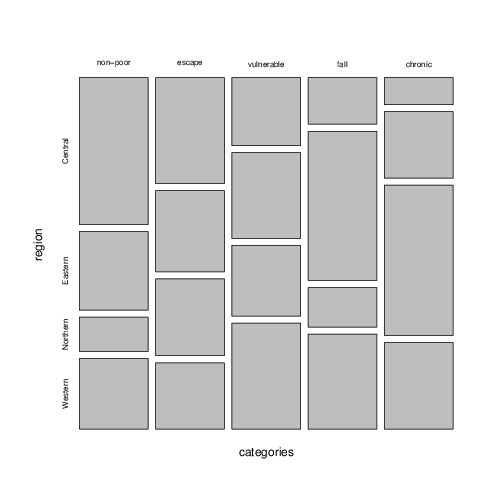
\includegraphics[scale=0.7]{/home/bjvca/data/data/GAP/Haruna/regionalprof}
\par\end{centering}

\centering{}Source: Author's calculations from the UNPS. 
\end{figure}


As mentioned above, location also affects access to services, such
as safe drinking water. Figure \ref{fig:Time-to-fetch} provides kernel
density plots for time reported to fetch drinking water including
waiting time. You can see that respondents cluster their answers around
2 hours and 4 hours. We find that, in general, the non-poor need to
spend less time fetching water, except maybe for some non-poor that
spend about 2 hours. The median for the non-poor is about 50 minutes,
as opposed to about 60 minutes for the chronic poor. The respective
means are 63 minutes for the non-poor and 77 for the poor. This is
also illustrated by the fact that the chronic poor have higher densities
at the extreme right of the distribution, for instance around 4 hours,
or 240 minutes. The vulnerable have a high density around 2 hours.

\begin{figure}
\protect\caption{Time to fetch water\label{fig:Time-to-fetch}}


\begin{centering}
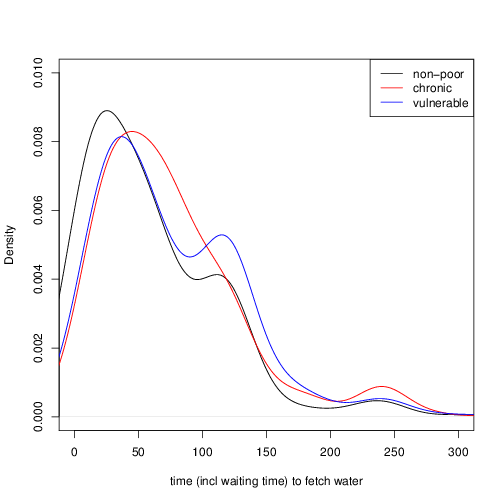
\includegraphics[scale=0.7]{/home/bjvca/data/data/GAP/Haruna/watertime}
\par\end{centering}

\centering{}Source: Author's calculations from the UNPS. 
\end{figure}



\subsection{Household demographics}

The size and composition of the household are also variables that
often feature in poverty regressions. For instance, many studies find
that household size is a good poverty indicator. It is thought that
increased competition for a given food stock reduces consumption.
However, \citet{RePEc:ecj:econjl:v:105:y:1995:i:433:p:1415-34} argue
that the negative correlation disappears as one takes economies of
scale in household food consumption into account. In terms of production,
a larger household may mean more and cheaper labor is available, but
\citet{newbjorn} finds that especially mothers in larger households
devote a significant amount of time to non-productive activities.
This last feature may be captured better when using relating the different
types of household in terms of poverty dynamics to dependency ratios.

Female-headedness is also often found to be a good predictor of poverty.
The underlying reasons should be sought in differences between male-headed
and female-headed households in terms of access to secure land tenure,
labor, credit, technology, and extension services (e.g. \citealt{Quisumbing2010581}).
One of the consequences is that female-headed households employ fewer
inputs, such as improved seeds and fertilizer, which has been shown
to reduce productivity (e.g. \citealt{Udry1995407}). We will also
look at marital status as an alternative way to look at gender-based
agricultural gaps. This will enable us to see if, for instance, widowhood
is associated with chronic poverty (\citealt{vandeWalle20131}). 

We find that indeed, chronic poor households are more likely to be
headed by a female. In addition, households that were never poor in
our panel, as well as households that are escaping poverty over time,
are more likely to be headed by a male. For the other categories,
we do not find big differences between male- and female-headed households.
We also looked at the age of the household head. We find that average
age of the household head is around 40 for households that are chronic
poor or have been sliding into poverty. Households that have never
been poor or that have moved out of poverty are on average about 4
years older. 

Figure \ref{fig:Poverty-Dynamics-and} gives an idea of the distribution
household size and child dependency ratios conditional on the poverty
dynamics group of the household. In the left panel (1), we plot box
plots for household size for each of the five poverty dynamics classes.
In the right panel (2) we do the same for child dependency ratios.
For each household we calculate the share of children under the age
of 15 within the total household and use this to plot box plots by
poverty dynamics category. We find that higher child dependency is
associated with chronic poverty, while the non-poor have the lowest
median child dependency ratio. Looking at both of the charts together,
the chronic poor have relatively large households and high dependency
ratios. Those that are never poor have small households and low dependency
ratios. Households that slide below the poverty threshold and those
that are vulnerable have a surprisingly high dependency ratio given
the relatively smaller households. These may be households where one
of the parents has died or has left the household. Large households
with a high dependency ratio also escape poverty. These may be households
that start to benefit from the additional cheap labor provided by
children. 

\begin{figure}
\protect\caption{Household size and child dependency ratios\label{fig:Poverty-Dynamics-and}}


\begin{centering}
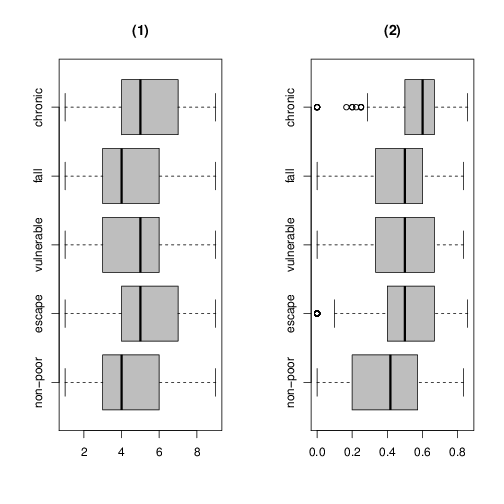
\includegraphics[scale=0.7]{/home/bjvca/data/data/GAP/Haruna/dependency}
\par\end{centering}

\centering{}Source: Author's calculations from the UNPS. 
\end{figure}


For marital status of the household head, respondents could choose
from five mutually exclusive types of marriage: married monogamously,
married polygamously, divorced, widow or widower, and never married.
The results are presented as a table of proportions where the rows
sum to 1 (Table \ref{tab:Marital-status}). This allows us to judge
the fraction of the total in each type of marriage accounted for by
each of our poverty transition groups. Thus, although the chronic
poor account for only about 12.3 per cent of the population, they
account for almost 20 per cent of individuals living in households
where the head has never been married. However, at the same time,
households where the head is never married are clearly more likely
to be non-poor, as are households where the head has divorced. We
also see that widowed households are underrepresented in the non-poor
segment. In addition, households headed by widows appear to have a
hard time keeping consumption smooth, as is evident by the large proportion
classified as vulnerable. Divorced household heads have been more
successful in moving out of poverty and are underrepresented in the
group of chronic poor households. Polygamously married households
have been less successful in escaping poverty. Just as widowed household
heads, they seem to have a hard time keeping consumption smooth between
the different years.

\begin{table}
\protect\caption{Marital status\label{tab:Marital-status}}


\begin{centering}
\begin{tabular}{lccccc}
\hline 
 & Non-poor & Escape & Vulnerable & Fall & Chronic\tabularnewline
\hline 
Married monogamously & 0.367 & 0.192 & 0.230 & 0.086 & 0.125\tabularnewline
Married polygamously & 0.348 & 0.152 & 0.299 & 0.081 & 0.119\tabularnewline
Divorced & 0.420 & 0.238 & 0.169 & 0.077 & 0.096\tabularnewline
Widowed & 0.272 & 0.246 & 0.293 & 0.071 & 0.118\tabularnewline
Never married & 0.517 & 0.125 & 0.139 & 0.029 & 0.190\tabularnewline
 &  &  &  &  & \tabularnewline
All & 0.358 & 0.190 & 0.247 & 0.082 & 0.123\tabularnewline
\hline 
\end{tabular}
\par\end{centering}

\centering{}Source: Author's calculations from the different waves
of the UNPS.
\end{table}



\subsection{Activity}

Table \ref{tab:activities} looks at what households report to be
their major source of earnings at the beginning of the panel. While
in general 35.8 per cent of Ugandans fall in the non-poor category,
only 25.7 per cent of the Ugandan subsistence farmers are in the non-poor
subgroup. It seems the group of vulnerable households is disproportionately
represented within the group of subsistence farmers. Subsistence farming
is indeed a very risky activity, and subsistence farmers have few
assets to insure against adverse shocks such as bad weather outcomes
or disease. Individuals that are living in households that report
to be engaged in commercial farming appear more likely to be non-poor.
Wage employment also seems to be an activity that is prevalent among
the non-poor. But among the wage employed, there is also an over-representation
in the group of people that have fallen into poverty.

\begin{table}
\protect\caption{Most important source of earnings\label{tab:activities}}


\begin{centering}
\begin{tabular}{lccccc}
\hline 
 & Non-poor & escape & vulnerable & fall & chronic\tabularnewline
\hline 
Subsistence farming & 0.257 & 0.211 & 0.293 & 0.089 & 0.150\tabularnewline
Commercial farming & 0.563 & 0.160 & 0.258 & 0.019 & 0.000\tabularnewline
Wage employment & 0.513 & 0.145 & 0.152 & 0.094 & 0.097\tabularnewline
Non-agricultural enterprises & 0.535 & 0.159 & 0.160 & 0.060 & 0.086\tabularnewline
Property income & 0.865 & 0.035 & 0.037 & 0.064 & 0.000\tabularnewline
Transfers & 0.555 & 0.207 & 0.168 & 0.048 & 0.021\tabularnewline
Organizational support  & 0.172 & 0.132 & 0.290 & 0.057 & 0.349\tabularnewline
 &  &  &  &  & \tabularnewline
All & 0.358 & 0.190 & 0.247 & 0.082 & 0.123\tabularnewline
\hline 
\end{tabular}
\par\end{centering}

\centering{}Source: Author's calculations from the different waves
of the UNPS.
\end{table}


Ugandans engaged in nonagricultural enterprises are also likely to
fall into the non-poor category. The most clear results are for those
who mention their main source of income is property - virtually all
are non-poor. People that depend on transfers are also non-poor. Transfers
are likely to correlate with social capital, and hence the lower probability
that households fall into the vulnerable group or in the group that
falls into poverty. Finally, a significant group of people reported
to be depending on handouts. As expected, these are especially the
chronic poor or individuals that are vulnerable. It is, however, also
interesting to note that 17.2 per cent of the individuals that report
organizational support as their main source of income are never poor
in the four-wave panel.


\subsection{Education}

In traditional poverty profiles, the education level of the household
head is often significant. Indeed, skills are important for the self-employed,
and schooled labor is likely to be better rewarded. It is less obvious
how schooling affects poverty dynamics in the short run. Lack of education
has been linked to intergenerational poverty (\citealt{Harper2003535}).
Education is also among the initial characteristics associated with
chronic poverty in rural communities in Ethiopia (\citealt{doi:10.1080/00220388.2011.625410}). 

Table \ref{tab:eduhead} looks at the highest education level reported
by the household head. We see that 17.6 per cent of all Ugandan household
heads have never attended school. However, within the group of individuals
in households that have always been poor, the share of households
that are headed by someone without formal education is 37 per cent.
On the other hand, the share of household with heads without schooling
in the subgroup of the non-poor is only 7.8 per cent. In the second
row, we see that the majority of household heads have finished primary
eduction. Primary education also seems insufficient to keep the household
permanently out of poverty. Everything above primary education leads
to a higher-than-average chance to be in the non-poor class. 

\begin{sidewaystable}
\protect\caption{Education of household head\label{tab:eduhead}}


\begin{centering}
\begin{tabular}{lccccccc}
\hline 
 & non-poor & Escape & Vulnerable & Fall & Chronic &  & All\tabularnewline
\hline 
No schooling  & 0.078 & 0.190 & 0.227 & 0.142 & 0.366 &  & 0.176\tabularnewline
Primary & 0.425 & 0.648 & 0.627 & 0.642 & 0.583 &  & 0.554\tabularnewline
Post-primary training/certificate & 0.085 & 0.026 & 0.024 & 0.032 & 0.010 &  & 0.045\tabularnewline
Secondary & 0.297 & 0.119 & 0.114 & 0.175 & 0.041 &  & 0.177\tabularnewline
Post-secondary training/certificate & 0.086 & 0.016 & 0.006 & 0.009 & 0.000 &  & 0.036\tabularnewline
Above & 0.029 & 0.000 & 0.002 & 0.000 & 0.000 &  & 0.011\tabularnewline
\hline 
\end{tabular}
\par\end{centering}

\centering{}Source: Author's calculations from the different waves
of the UNPS.
\end{sidewaystable}



\subsection{Health}

Illness and health shocks have been reported to affect poverty dynamics.
For instance, \citet{doi:10.1080/00220380500405394} note that serious
human health shocks causing permanent injury or illness or death were
among the most frequently cited reasons for households falling into
poverty in quantitative data from Madagascar and Kenya. But the bidirectional
nature of the poverty relationship between poverty and health may
trap households in persistent poverty, as ill health can be a catalyst
for poverty spirals and in turn poverty can create and perpetuate
poor health status (\citealt{grant}).

Health status is likely to be a function of the distance the nearest
health facility. Figure \ref{fig:Distance-to-health} reports on distance
to nearest health facility. By health facility we mean either a private
clinic, a government or non-governmental health unit or hospital.
There seems to be some pattern in the data. Households that are never
poor in any of the waves of the panel dataset reported lowest median
distance to health facilities. At the other extreme, we find that
households that live in chronic poverty reported highest median distance
to health facilities. Distance to health facilities likely reflects
location, as we have seen that the chronic poor tend to live in more
remote areas.

\begin{figure}
\protect\caption{Distance to health infrastructure\label{fig:Distance-to-health}}


\begin{centering}
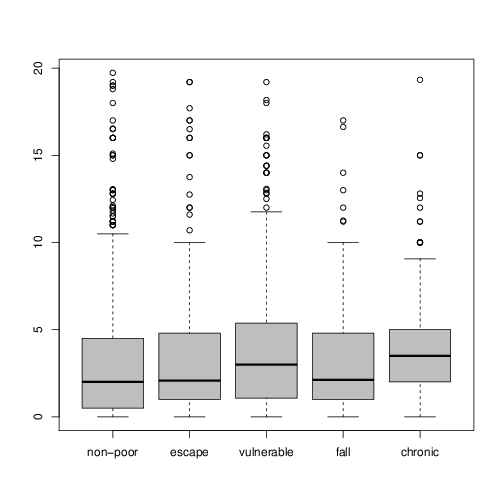
\includegraphics[scale=0.7]{/home/bjvca/data/data/GAP/Haruna/distance_health}
\par\end{centering}

\centering{}Source: Author's calculations from the UNPS. 
\end{figure}


Figure \ref{fig:Days-inactive} looks at average days that household
heads reported being inactive due to illness in the last six months
in the 2005/06 UNPS wave conditional on subsequent poverty transitions.
For most of the categories, the number of days lost is on average
about 8.5 days. We see that people that have lost relatively few days
due to illness are more likely to be in the subgroup that subsequently
escapes poverty. On the other hand, the households that report the
highest number of days lost by the household head due to illness are
those that are in the subgroup of households that eventually fall
into poverty or are living in chronic poverty.

\begin{figure}
\protect\caption{Days inactive\label{fig:Days-inactive}}


\begin{centering}
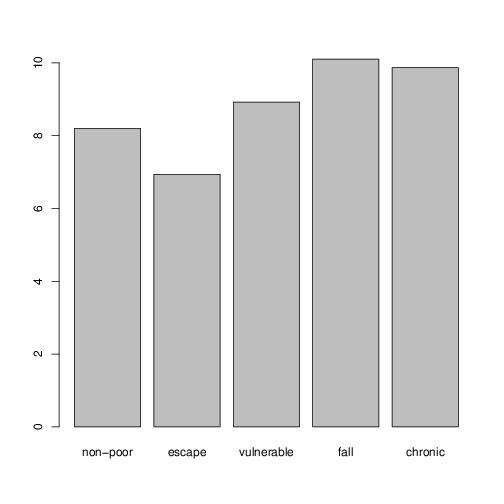
\includegraphics[scale=0.7]{/home/bjvca/data/data/GAP/Haruna/days_inactive}
\par\end{centering}

\centering{}Source: Author's calculations from the UNPS. 
\end{figure}



\subsection{Shocks and Coping}

The poor are known to be more vulnerable to shocks, due to their lower
ability to insure (\citealt{RePEc:oxp:obooks:9780199276837}). Shocks
can have lasting effects if they destroy productive assets, such as
when droughts reduce livestock, or health shocks that destroy human
capital. If households are left with too few productive assets to
replenish the gap left by shocks, they are likely to fall into an
asset-based poverty trap (\citealt{doi:10.1080/00220380500405261}).
We also look at how the households deal with shocks ex post conditional
on their wealth dynamics category.

Table \ref{tab:shocks} look at shocks reported at the onset of the
panel. We again report column percentages. Hence, while 35 per cent
of all shocks are drought related, this increases to almost 40 per
cent in the group of the chronic poor. Still, drought also features
prominently in the group that subsequently escapes poverty. A substantial
share of the non-poor report to have been exposed to drought shocks,
but this share is only about 5 percentage points lower than the overall
share that reports drought-related shocks. Floods, hailstorms, and
also pest reports do not seem to differ too much between the different
groups.

Bad seed quality is reported more among the non-poor than average.
This may be because especially farmers that are always above the poverty
line are more commercially oriented and buy seed, instead of recycling
seeds. As such, they are also more prone to counterfeit seeds. But
probably the most significant result in this table is the disproportionate
number of people within chronically poor households that report being
affected by civil strife. Poverty that is associated with civil war
seems to be very persistent (\citealt{RePEc:eee:wdevel:v:31:y:2003:i:3:p:629-646}).
The non-poor clearly faced different shocks. They report more than
average losses related to robbery and theft. This category also shows
up relatively more in the category of households that slide into poverty.
The death of a family member is also disproportionately mentioned
among those that fall into poverty over the period covered by the
panel.

\begin{sidewaystable}
\protect\caption{Shocks\label{tab:shocks}}


\begin{centering}
\begin{tabular}{lccccccc}
\hline 
 & non-poor & Escape & Vulnerable & Fall & Chronic &  & All\tabularnewline
\hline 
Drought & 0.302 & 0.383 & 0.369 & 0.350 & 0.388 &  & 0.350\tabularnewline
Floods/hailstorm & 0.125 & 0.135 & 0.136 & 0.114 & 0.129 &  & 0.129\tabularnewline
Pest attacks & 0.098 & 0.086 & 0.084 & 0.098 & 0.082 &  & 0.090\tabularnewline
Bad seeds quality & 0.035 & 0.011 & 0.023 & 0.021 & 0.018 &  & 0.024\tabularnewline
Livestock epidemic & 0.065 & 0.067 & 0.042 & 0.047 & 0.061 &  & 0.057\tabularnewline
Fire accident & 0.018 & 0.021 & 0.036 & 0.024 & 0.038 &  & 0.027\tabularnewline
Civil strife & 0.037 & 0.059 & 0.074 & 0.051 & 0.123 &  & 0.064\tabularnewline
Robbery/theft & 0.102 & 0.055 & 0.075 & 0.098 & 0.063 &  & 0.081\tabularnewline
Death of the head of the household & 0.022 & 0.041 & 0.023 & 0.028 & 0.023 &  & 0.026\tabularnewline
Death of other family member & 0.139 & 0.097 & 0.107 & 0.123 & 0.038 &  & 0.108\tabularnewline
Injury from accidents & 0.033 & 0.011 & 0.010 & 0.024 & 0.010 &  & 0.019\tabularnewline
Other & 0.024 & 0.032 & 0.020 & 0.021 & 0.025 &  & 0.024\tabularnewline
\hline 
\end{tabular}
\par\end{centering}

\centering{}Source: Author's calculations from the different waves
of the UNPS.
\end{sidewaystable}


Finally, the dot chart in figure \ref{fig:Coping-with-Adverse} shows
how the different categories of households reportedly dealt with shocks.
The top of the chart shows that the non-poor most often used savings
to cope with shocks. This is also reported as a main source of ex-post
insurance for a substantial part that have slid into poverty over
the course of the panel. The chronic poor deal in a completely different
way with shocks. For instance, they can not rely on savings to deal
with shocks. Instead, the poor seem to rely on employment and migration,
but most of all simply have no choice but to reduce consumption. The
graph also shows the importance of social capital to deal with shocks
for vulnerable households. There is also some indication that informal
borrowing during the first round of our panel is associated to an
increase in the chance that households descend into poverty.

\begin{figure}
\protect\caption{Coping with adverse shocks\label{fig:Coping-with-Adverse}}


\begin{centering}
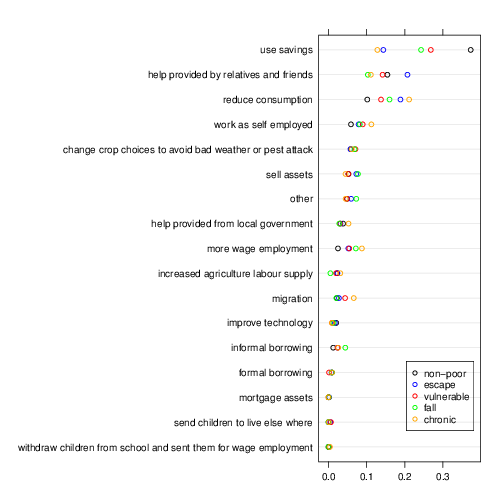
\includegraphics[scale=0.7]{/home/bjvca/data/data/GAP/Haruna/coping_fin}
\par\end{centering}

\centering{}Source: Author's calculations from the UNPS. 
\end{figure}



\section{Conclusion}

In this paper, we reassess the evolution of poverty over the past
ten years in Uganda. Official figures suggest substantial poverty
reduction, but independent researchers note that the benefits of economic
growth have been shared unequally. In addition, casual observation
does not correspond to the rosy picture that official figures suggest.
Other indicators that define well-being in a broader way, such as
adult literacy and maternal health, also put Uganda at a much lower
level than what would correspond to the disseminated poverty levels. 

One possible explanation for this divergence lies in the poverty line.
The poverty line that is currently in use to estimate official poverty
in Uganda was constructed more than a decade ago, using data from
a 1993/1994 survey. In addition, this poverty line relies on a single
food consumption basket for Uganda, despite the fact that Uganda consists
of a diverse set of regions, each with their own diets. These diets
are also exceptional in their difference in cost to obtain a certain
level of kilo-calories (or utility of that matter). Lumping all regions
together and assuming they require the same amounts of each commodity
disregards the cultural and agro-climatic diversity that typifies
Uganda.

We therefore follow \citet{RePEc:ucp:ecdecc:v:58:y:2010:i:3:p:449-474},
who propose an information-theoretic approach to constructing utility-consistent
poverty lines. The idea is to construct different poverty lines by
spatial (or temporal) domain that yield a minimal amount of kilo-calories
given the demographic makeup of the region. These poverty lines are
then tested to check if they obey revealed preference conditions.
In particular, we check if the food baskets chosen in all other regions
are less expensive than the food basket chosen in a particular region.
If not, the individual could have chosen a cheaper basket that yields
the same utility. This violates the revealed preference condition.
We apply an information-theoretic approach that adjusts consumption
shares such that this revealed preference condition is satisfied,
while keeping the original diets intact as much as possible.

We feel that the poverty estimates using poverty lines that reflect
local diets are more realistic than the official ones. For instance,
they are much more in line with the levels and evolution of other
non-monetary poverty indicators. A case in point is the nutritional
status of children. According to the Uganda Demographic Household
Survey 2011, height-for-age scores are worst in the western region,
except for the Karamoja district. \citet{RePEc:ags:eprcrs:113614}
also find that the highest rates of stunting are in the southwestern
subregion. This at least indicates that the situation in terms of
poverty is less rosy than official figures suggest.

While our analysis shows the situation has improved over time in the
northern region, a disturbingly large proportion of the chronic poor
remain. In addition, a substantial proportion of vulnerable households
resides in the northern region. The use of utility-consistent poverty
lines that are allowed to differ in terms of diet by geographic location
also points to substantial poverty in the western region. The fact
that in this region, relatively few households are escaping poverty
and relatively more households are falling into poverty needs attention.
This is in stark contrast to the central region, where, despite the
already high presence of non-poor, many poor households have escaped
poverty over time and very few households have slipped back into poverty.

Turning to household demographics, we find that chronic poor households
are more likely to be headed by a female. In addition, households
that were never poor in our panel are more likely to be headed by
a male. Higher child dependency is associated with chronic poverty,
while the non-poor have the lowest median child dependency ratio.
Despite the relatively low household size, it now seems that the households
that slide below the poverty threshold have a surprisingly high dependency
ratio. These may be households where one of the parents has died or
has left the household. We also see that widowed households are underrepresented
in the non-poor segment. In addition, households headed by widows
appear to have a hard time keeping consumption smooth, as is evident
by the large proportion classified as vulnerable. Households where
the head is never married are clearly more likely to be non-poor.
Divorced household heads have been more successful in moving out of
poverty, and they are also more likely to be non-poor. Polygamously
married households have been disproportionately sliding into poverty
and are also slightly more likely to be chronic poor.

If we look at the main source of income at the start of the panel,
we find a significant group of people that reported to be depending
on handouts. As expected, these are especially the chronic poor or
individuals that fall into poverty. It seems the group of vulnerable
households is disproportionately represented within the group of subsistence
farmers, underlining the riskiness of rain-fed agriculture. Ugandans
engaged in commercial agriculture of non-agricultural enterprises
are also likely to fall into the non-poor category.

We then look at education and health. We find that households that
live in chronic poverty reported highest median distance to health
facilities. Distance to health facilities likely reflects location,
as we have seen that the chronic poor tend to live in more remote
areas. Another striking feature is that long periods of illness (in
terms of days lost due to illness) are correlated with sliding into
poverty. Primary education of the household head alone also seems
insufficient to escape poverty in the long run. Finally, we find some
interesting results with respect to shocks and how households subsequently
deal with these shocks. While the chronic poor have no other option
than to reduce consumption, the non-poor draw on savings. Social networks
also seem important for vulnerable households.

\newpage{}\bibliographystyle{/home/bjvca/IFPRI_Style}
\bibliography{gap_paper}


\newpage{}


\section*{Appendix}

\setcounter{table}{0} \renewcommand{\thetable}{A.\arabic{table}} 

\begin{table}[H]
\protect\caption{Utility-consistent poverty lines \label{tab:Utility-Consistent-Poverty}}


\begin{centering}
\begin{tabular}{lcccccc}
\hline 
 & \multicolumn{1}{c}{2005/06} & \multicolumn{1}{c}{2009/10} & 2010/11 & 2011/12 & 2012/13 & foodshare\tabularnewline
\hline 
National & 616.09 & 887.09 & 945.03 & 1167.38 & 1233.42 & 0.72\tabularnewline
 &  &  &  &  &  & \tabularnewline
Kampala & 1262.39 & 1817.68 & 1936.38 & 2392.00 & 2527.30 & 0.62\tabularnewline
central Rural & 1029.78 & 1482.75 & 1579.58 & 1951.24 & 2061.62 & 0.68\tabularnewline
Eastern Rural & 765.61 & 1102.38 & 1174.37 & 1450.68 & 1532.75 & 0.71\tabularnewline
Northern rural & 900.38 & 1296.43 & 1381.09 & 1706.05 & 1802.56 & 0.72\tabularnewline
Western Rural & 973.32 & 1401.46 & 1492.99 & 1844.27 & 1948.60 & 0.72\tabularnewline
Other Urban & 983.16 & 1415.62 & 1508.07 & 1862.90 & 1968.28 & 0.69\tabularnewline
\hline 
\end{tabular}
\par\end{centering}

\centering{}Source: Figures are calculated from the respective UNHS
and UNPS waves. 
\end{table}


\begin{table}[H]
\protect\caption{Poverty gap 2002-2012 using six spatial domains\label{tab:Poverty-gap-2002-2012}}


\begin{centering}
\begin{tabular}{lcccccccccc}
\hline 
 & \multicolumn{2}{c}{2005/06} & \multicolumn{2}{c}{2009/10} & \multicolumn{2}{c}{2010/11} & \multicolumn{2}{c}{2011/12} & \multicolumn{2}{c}{2012/13}\tabularnewline
 & P1 & contr & P1 & contr & P1 & contr & P1 & contr & P1 & contr\tabularnewline
\hline 
\hline 
National & 0.143 & 1.000 & 0.133 & 1.000 & 0.131 & 1.000 & 0.106 & 1.000 & 0.092 & 1.000\tabularnewline
 &  &  &  &  &  &  &  &  &  & \tabularnewline
Rural & 0.162 & 0.946 & 0.151 & 0.952 & 0.146 & 0.959 & 0.119 & 0.936 & 0.104 & 0.872\tabularnewline
Urban & 0.047 & 0.054 & 0.040 & 0.048 & 0.039 & 0.041 & 0.040 & 0.064 & 0.051 & 0.128\tabularnewline
 &  &  &  &  &  &  &  &  &  & \tabularnewline
Central & 0.092 & 0.198 & 0.077 & 0.177 & 0.050 & 0.096 & 0.031 & 0.064 & 0.032 & 0.092\tabularnewline
Eastern & 0.101 & 0.175 & 0.090 & 0.165 & 0.107 & 0.219 & 0.092 & 0.279 & 0.085 & 0.270\tabularnewline
Northern & 0.302 & 0.364 & 0.242 & 0.327 & 0.197 & 0.347 & 0.193 & 0.381 & 0.221 & 0.499\tabularnewline
Western & 0.139 & 0.262 & 0.165 & 0.331 & 0.179 & 0.337 & 0.116 & 0.276 & 0.053 & 0.139\tabularnewline
\hline 
\end{tabular}
\par\end{centering}

\begin{centering}
Source: Figures are calculated from the respective UNHS and UNPS waves. 
\par\end{centering}

\centering{}Note: P1 means poverty gap ratio, contr means contribution
to national poverty. 
\end{table}


\begin{table}[H]
\protect\caption{Poverty severity 2002-2012 using six spatial domains\label{tab:Poverty-severity-2002-2012}}


\begin{centering}
\begin{tabular}{lcccccccccc}
\hline 
 & \multicolumn{2}{c}{2005/06} & \multicolumn{2}{c}{2009/10} & \multicolumn{2}{c}{2010/11} & \multicolumn{2}{c}{2011/12} & \multicolumn{2}{c}{2012/13}\tabularnewline
 & P2 & contr & P2 & contr & P2 & contr & P2 & contr & P2 & contr\tabularnewline
\hline 
\hline 
National & 0.066 & 1.000 & 0.063 & 1.000 & 0.063 & 1.000 & 0.046 & 1.000 & 0.040 & 1.000\tabularnewline
 &  &  &  &  &  &  &  &  &  & \tabularnewline
Rural & 0.075 & 0.949 & 0.072 & 0.951 & 0.071 & 0.962 & 0.051 & 0.929 & 0.045 & 0.867\tabularnewline
Urban & 0.020 & 0.051 & 0.019 & 0.049 & 0.017 & 0.038 & 0.019 & 0.071 & 0.023 & 0.133\tabularnewline
 &  &  &  &  &  &  &  &  &  & \tabularnewline
Central & 0.041 & 0.191 & 0.036 & 0.174 & 0.026 & 0.106 & 0.010 & 0.049 & 0.011 & 0.075\tabularnewline
Eastern & 0.037 & 0.141 & 0.039 & 0.148 & 0.041 & 0.174 & 0.035 & 0.244 & 0.031 & 0.227\tabularnewline
Northern & 0.164 & 0.430 & 0.126 & 0.356 & 0.100 & 0.366 & 0.095 & 0.434 & 0.111 & 0.582\tabularnewline
Western & 0.058 & 0.238 & 0.076 & 0.322 & 0.091 & 0.354 & 0.049 & 0.273 & 0.019 & 0.116\tabularnewline
\hline 
\end{tabular}
\par\end{centering}

\begin{centering}
Source: Figures are calculated from the respective UNHS and UNPS waves. 
\par\end{centering}

\centering{}Note: P2 means severity of poverty measure, contr means
contribution to national poverty. 
\end{table}

\end{document}
